For the training process, we deliberately use NCSM calculations which are calculated to a sufficiently high $N_\mathrm{max}$, to extract the limit as a prediction target for the networks. In our basic training mode, the sequences further get divided into subsequences of four consecutive $N_\mathrm{max}$ values. The network then gets trained to predict the same limit value for all of those subsequences. Since there are very high $N_\mathrm{max}$ values available, the training set of input sequences also contains sequences with almost constant values, as the sequences have already converged enough to the limit value at that model-space dimension. The result in the network also getting trained on converged sequences, for which there is no extrapolation needed. In \autoref{fig:example_nmax}, we can see an example sequence which will be used in training. It is clear that sequences above $N_\mathrm{max} \approx 26$ are almost converged and thus provide no new insights for the network about how to extrapolate unconverged sequences. Furthermore, those sequences might even prevent the networks from extrapolating unconverged sequences, as the networks could learn to just reproduce the lowest value of the sequence, as is the case for the converged sequences.

In order to conform to the later use-cases of the extrapolation of unconverged sequences, we should also focus our training on the extrapolation of those sequences. To achieve this, we want to restrict the input sequences to lower values of $N_\mathrm{max}$. As we can already see in \autoref{fig:example_nmax}, a restriction of subsequences to a maximum $N_\mathrm{max}$ of 24 will lead to the exclusion of the extreme cases of converged sequences and an inclusion of high enough $N_\mathrm{max}$ values to allow for different convergence rates in the training set.
\begin{figure}[H]
  \centering
  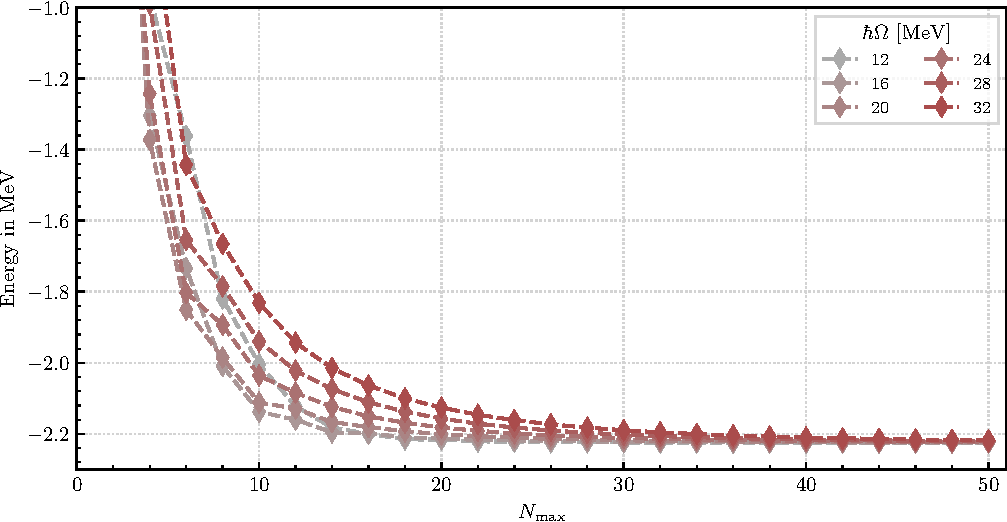
\includegraphics{media/example_sequence.pdf}
  \caption{NCSM results for the $\n{2}{H}$ nucleus. Here, the interaction used for the Hamiltonian is a chiral N$^{3}$LO interaction with two-body interactions and a cutoff at \SI{400}{\mega\electronvolt} by Entem, Machleidt and Nosyk \cite{entemmachleidt}. Furthermore, the Hamiltionian is SRG evolved using a flow parameter of $\SI{0.04}{\femto\metre^4}$. Each point is the result of a NCSM calculation with a given $N_\mathrm{max}$ and oscillator frequency $\hbar \Omega$.}
  \label{fig:example_nmax}
\end{figure}
